\section{Goals}
\begin{itemize}[label=$\bullet$, itemsep=-1pt, leftmargin=*]
	\item Students are familiar with and able to use logical and comparison expressions in the C programming language.
	\item Students are familiar with and able to use logical and comparison expressions in the C programming language.
	\item Students can recognize and use while loops in the C language.
	      % \item Students are able to use while-loop on C
	\item Students can recognize and use do-while loops in the C language.
	      % \item Students are able to use do-while loop on C
	\item Students can recognize and use for loops in the C language.
	      % \item Students are able to use for loop on C
	\item Students can recognize and use for loops in the C language.
	      % \item Students are able to use one dimensional or multidimensional array
	\item Students can recognize and use for loops in the C language.
	      % \item Students are able to use loops to process data on arrays
	\item Students can recognize and use strings.
\end{itemize}
\section{Logical and Comparasion Expressions}
\subsection{Comparasion Expressions}
% Berikut adalah operator-operator yang digunakan pada suatu ekspresi perbandingan
The following are the operators used in comparison expressions.
\begin{center}
	\captionof{table}{Comparasion Operator\label{tab:operatorcomp}}
	\begin{tabular}{|c|l|c|}
		\hline
		\textbf{Operator} & \textbf{Name}         & \multicolumn{1}{l|}{\textbf{Expression Example}} \\ \hline
		!=                & Not Equal To          & x != y                                           \\ \hline
		\textgreater{}    & Greater Than          & x \textgreater y                                 \\ \hline
		==                & Equal To              & x == y                                           \\ \hline
		\textless{}       & Less Than             & x \textless y                                    \\ \hline
		\textgreater{}=   & Greater Than Equal To & x \textgreater{}= y                              \\ \hline
		\textless{}=      & Less Than Equal To    & x \textless{}= y                                 \\ \hline
	\end{tabular}
\end{center}

% Suatu ekspresi perbandingan akan mengembalikan nilai berupa \verb|true| atau \verb|false| yang ditandakan dengan nilai 0 atau 1.
A Comparison Expression will return boolean value \verb|true| or \verb|false| which is also represented with the value 1 or 0.
As example:
\begin{verbatim}
    printf("%d",0>1); // Print 0 to the screen
    printf("%d",0<1); // Print 1 to the screen
\end{verbatim}

\subsection{Logical Expression}
% Berikut adalah operator-operator logika yang digunakan pada suatu ekspresi logika
The following are the logical operators used on a Logical Expression
\begin{center}
	\captionof{table}{Logical Expression \label{tab:operatorlogic}}
	\begin{tabular}{|c|l|c|}
		\hline
		Operator & \multicolumn{1}{c|}{Name} & Expression Example     \\ \hline
		$\&\&$   & AND                       & $x<5\; \&\& \;x<10$    \\ \hline
		$||$     & OR                        & $x < 5\; ||\; x < 4  $ \\ \hline
		$!$      & NOT                       & $!(x <5 \&\& x < 10) $ \\ \hline
	\end{tabular}
\end{center}
% Sama seperti ekspresi perbandingan, ekspresi logika akan mengembalikan nilai berupa true atau false
Like comparison expression, logical expression will return boolean values.

\section{Branch}
\subsection{If Statement}
\verb*|if| statement is used to decide which block of code to be executed if the condition is true.
% \verb*|if| digunakan untuk menentukan blok kode C yang dijalankan apabila ekspresi kondisi bernilai benar (TRUE),
\begin{verbatim}
// Block code before if
if (Condition) 
{
 // Block of code that will be executed if the condition is true
}
// Block code after if
\end{verbatim}
% Sebagai contoh, perhatikan program berikut
As example, look at the following code
\begin{lstlisting}[language=c,caption =If Statement Example,label=lst:ifexample01]
	include <stdio.h>
	
	int main()
	{
		//Variable Declaration
		int myMoney,breadPrice;
		myMoney = 5000;
		breadPrice = 10000;
		
		if (myMoney>=breadPrice)
		{
		    printf("I can buy that bread\n");
		}
		printf("hehe");
		return 0;
	}
\end{lstlisting}
Output of the program
\begin{verbatim}
    hehe
\end{verbatim}
If line 7 changed to \verb|myMoney=10000|, the outputs of the program would be
% Jika baris ke 7 diganti dengan \verb|myMoney=10000| maka output dari program ini akan menjadi
\begin{verbatim}
    I can buy that bread
    hehe
\end{verbatim}

\subsection{If-else Statement}
% Pernyataan else digunakan untuk menentukan blok kode yang di jalankan apabila kondisi salah. 
Else statement is used to decide the block of code to be executed if the condition is false.
\begin{verbatim}
// Block code before if
if (Condition) 
{
	// Block of code that will be executed if the condition is true
} else
{
	// Block of code that will be executed if the condition is false
}
// Bloc code after if-else
\end{verbatim}
% Berikut contoh penggunaan if-else
The following is an example of using if-else statement:
\begin{lstlisting}[language=c,caption = If-else example,label=lst:ifelseexample01]
	include <stdio.h>
	
	int main()
	{
		//Varible declaration
		int myMoney,breadPrice;
		myMoney = 5000;
		breadPrice = 10000;
		
		if (myMoney>=breadPrice)
		{
		    printf("I can buy that bread\n");
		}
		else
		{
	        printf("I can't buy that bread\n");	
		}
		printf("hehe");
		return 0;
	}
\end{lstlisting}
Below is the output of that program
\begin{verbatim}
    I can buy that bread
    hehe
\end{verbatim}
%  \verb|myMoney=10000| maka output dari program ini akan menjadi
If line 7 changed to \verb|myMoney=10000|, the outputs of the program would be
\begin{verbatim}
    I can't buy that bread
    hehe
\end{verbatim}

\subsection{Pernyataan if-else if}
% Statement \verb|else if| digunakan untuk menjalankan blok kode apabila kondisi statement \verb|if| atau \verb|else if| sebelumnya bernilai salah.
The \verb|else if| statement is used to run a block of code when the condition in \verb|if| or the previous \verb|else if| is false.
\begin{verbatim}
	// Code block before the if statement
if (Condition1)
{
    /* Code block to be executed if Condition 1
    is true */
}
else if (Condition2)
{
    /* Code block to be executed if Condition 1 is false
    and Condition 2 is true */
}
else if (Condition3)
{
    /* Code block to be executed when
    Condition 1 and Condition 2 are false, and
    Condition 3 is true */
}
...
else if (ConditionN)
{
    /* Code block to be executed when
    Condition 1 to Condition N-1 are false, and
    Condition N is true */
}
else
{
    /* Code block to be executed when
    Condition 1 to Condition N are false */
}
// Code block after the if statement
\end{verbatim}
Below are an example of if-else statement
\begin{lstlisting}[language=c,caption = If-else example if,label=lst:ifelseifexample01]
	include <stdio.h>
	
	int main()
	{
		//Varible declaration
		int myMoney,breadPrice;
		myMoney = 5000;
		breadPrice = 10000;
		
		if (myMoney>breadPrice)
		{
		    printf("I can buy that bread\n");
		}
		else if(myMoney==breadPrice)
		{
		    printf("I can buy bread, but my money will run out immediately");
		}
		else
		{
	        printf("I can't buy that bread\n");	
		}
		printf("hehe");
		return 0;
	}
\end{lstlisting}
Output of this program are below
\begin{verbatim}
    I can't buy that bread
    hehe
\end{verbatim}
% Jika baris ke 7 diganti dengan \verb|myMoney=10000| maka output dari program ini akan menjadi
If line 7 changed to \verb|myMoney=10000|, the output of the program would be
\begin{verbatim}
    I can buy bread, but my money will run out immediately
    hehe
\end{verbatim}
% Jika baris ke 7 diganti dengan \verb|myMoney=12000| maka output dari program ini akan menjadi
If line 7 changed to \verb|myMoney=12000|, the output of the program would be
\begin{verbatim}
    I can buy that bread
    hehe
\end{verbatim}

\subsection{Nested if}
% Nested if merupakan konsep di mana di dalam suatu blok if terdapat statement if.
Nested if is when there is a conditional statements within a block of code inside the conditional statement
\begin{verbatim}
	// Code block before the if statement
	if (Condition1) 
	{
		if (Condition2)
		{
			// Do something
		}
		else
		{
			// Do other thing
		}
	} 
	else
	{
		// Do other thing
	}
\end{verbatim}

% Berikut contoh penggunaan nested if
Below is an example of using nested if

\begin{lstlisting}[language=c,caption = Nested if example,label=lst:nestedifexample01]
	include <stdio.h>
	
	int main()
	{
		// Declare the variables
		int myMoney,breadPrice,friendsMoney;
		myMoney = 5000;
		breadPrice = 10000;
		friendsMoney = 42069;
		
		
		if (myMoney>breadPrice)
		{
		    printf("I can buy bread\n");
		}
		else if(myMoney==breadPrice)
		{
		    printf("I can buy bread but I will ran out of money\n");
		}
		else
		{
		    if(friendsMoney+myMoney >= breadPrice)
		    {
		        printf("I can buy bread if I borrow my friend money\n"); 
		    }
		    else
		    {
	            printf("I can't buy bread\n");	
		    }
		}
		printf("hehe");
		return 0;
	}
\end{lstlisting}


\subsection{Pre-lab Assignment}
\begin{enumerate}
	% \item Buatlah program yang menerima input 3 buah bilangan bulat A, B, dan C. Outputkanlah 3 bilangan bulat itu ke layar dengan urutan paling kecil ke paling besar. Lakukanlah ini dengan menggunakan statement if, if else, if else if, atau nested if.
	\item Try to make a program that receives 3 integer input A, B, and C. Then outputs those 3 integers to the screen sorted from smallest to largest. Do this only using conditional statements.
\end{enumerate}

\section{Loop}
\subsection{Loop while}
% Perulangan while akan menjalankan blok kode yang berada di dalamnya selama kondisi perulangan masih bernilai benar.
While loop will run the code block within it repeatedly as long as the loop condition is true


\begin{figure}[H]
	\centering
	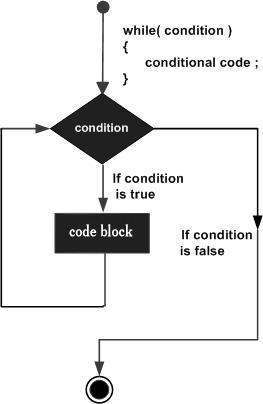
\includegraphics[width=0.4\linewidth]{P2/img/whileloop.png}
	\caption{Flow chart loop while}
	\label{fig:whileloop}
\end{figure}

% Syntaxnya pada bahasa C adalah sebagai berikut:
Its syntax in C programming language is as follows
\begin{verbatim}
    while(Condition)
    {
        // Block of code that will be repeated
    }
\end{verbatim}

% Sebagai contoh, perhatikan kode berikut
As an example, look at the following code
\begin{lstlisting}[language=c,caption = While implementation example,label=lst:whileexample01]
int main()
{
	int myMoney,breadPrice;
	myMoney = 10000;
	breadPrice = 2000;
	while(myMoney >= breadPrice)
	{
	    printf("Buy 1 bread, my money left %d", myMoney - breadPrice);
	    myMoney -= breadPrice;
	}
	printf("I don't have enough money");
	return 0;
}
\end{lstlisting}
Output in program \ref{lst:whileexample01} are below
\begin{verbatim}
    Buy 1 bread, my money left 8000
    Buy 1 bread, my money left 6000
    Buy 1 bread, my money left 4000
    Buy 1 bread, my money left 2000
    Buy 1 bread, my money left 0
    I don't have enough money
\end{verbatim}

% Pada contoh ini, operasi pada baris 9 membuat variabel \verb|myMoney| berkurang 2000 pada setiap pengulangan hingga akhirnya nilai \verb|myMoney| tidak lebih dari atau sama dengan \verb|breadPrice| lagi.
You can see the line 9 of the code causes the variable \verb|myMoney| to have its value substracted by 2000 for every loop until \verb|myMoney| is no longer greater than equal to \verb|breadPrice|.
The loop condition will be invalid and finaly exits the loop. Then it prints "Uang saya tidak cukup lagi", the command after the while loop statement.
% Kondisi perulangan akan menjadi tidak valid dan akhirnya keluar dari perulangan. Kemudian ia mencetak "Uang saya tidak cukup lagi", perintah setelah pernyataan while loop.
\subsection{Do-while loop}
% do-while loop sebenarnya sama seperti while loop hanya saja do-while akan menjalankan perintah pada blok kode didalamnya terlebih dahulu sebelum melakukan pengecekan kondisi.
do-while loop is very similar to while loop. The only difference is that do-while loop will execute the code block inside it once, and then checks the condition.
\begin{figure}[H]
	\centering
	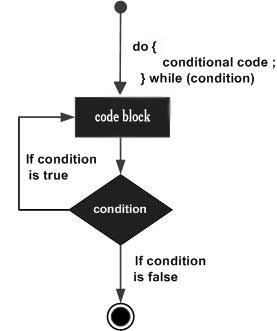
\includegraphics[width=0.4\linewidth]{P2/img/dowhileloop.png}
	\caption{Do-while statement}
	\label{fig:dowhileloop}
\end{figure}
% Syntaxnya pada bahasa C adalah sebagai berikut:
Its syntax in C is as follows:
\begin{verbatim}
    do{
        // the block of code that will be repeated
    }while(Condition)
\end{verbatim}
% Sebagai contoh, perhatikan kode berikut
Look at the following example.
\begin{lstlisting}[language=c,caption = Do-while implementation example,label=lst:dowhileexample01]
int main()
{
	int myMoney,breadPrice;
	myMoney = 10000;
	breadPrice = 12000;
	do{
	    printf("Buy 1 bread, my money left %d", myMoney - breadPrice);
	    myMoney -= breadPrice;
	}while(myMoney >= breadPrice)
	printf("Uang saya tidak cukup lagi");
	return 0;
}
\end{lstlisting}
The output of the code above in Listing \ref{lst:dowhileexample01} are
% The output of the code above are
\begin{verbatim}
    Buy 1 bread, my money -2000
    I don't have enough money
\end{verbatim}
The variable \verb|myMoney| is substracted by \verb|breadPrice| before checking the \verb|myMoney>=breadPrice| condition.
Had the code above uses while loop, the repeating block of code wouldn't have executed even once.
% Variabel \verb|myMoney| dikurangi dengan \verb|breadPrice| sebelum memeriksa \verb|myMoney>=breadPrice| kondisi.
% Seandainya kode di atas menggunakan perulangan while, blok kode yang berulang tidak akan dieksekusi sekali pun.
\subsection{For loop}
% Misalkan terdapat blok kode while dengan bentuk seperti ini:
If you have a block of code like this:
\begin{verbatim}
    InitializationStatement; // e.g.: int i = 0;
    while(Condition){
        // do something
        updateStatement; // e.g.: i++ 
    }
\end{verbatim}
This is equal to
\begin{verbatim}
    for(InitializationStatement;Condition;updateStatement){
        // do something
    }
\end{verbatim}

% Sebagai contoh, perhatikan program berikut:
As example, look at the following code:
\begin{lstlisting}[language=c,caption = For implementation example,label=lst:forexample01]
int main()
{
    int i=0;
    for(i=1;i<10;i++){
        printf("%d ",i);
    }
	return 0;
}
\end{lstlisting}
% Output dari program ini adalah
The output of this program are
\begin{verbatim}
    1 2 3 4 5 6 7 8 9 
\end{verbatim}
% Berikut kode pada Listing \ref{lst:forexample01} jika diubah menjadi bentuk while-loop
The following is the code if code in Listing \ref{lst:forexample01} converted to its while-loop form
\begin{lstlisting}[language=c,caption = For in form of while,label=lst:forwhileform01]
int main()
{
    int i=0;
    i=1;
    while(i<10){
        printf("%d ",i);
        i++;
    }
	return 0;
}
\end{lstlisting}
\begin{center}
	\colorbox{pink}{\parbox{0.8\linewidth}{\textbf{Notes:} In programming, the "break" keyword is used to exit a loop prematurely, while the "continue" keyword is used to skip the current iteration of a loop and proceed to the next iteration. These keywords are commonly used in loops to control their behavior and make the code more efficient. You can explore their usage further in programming resources and tutorials.!}}
\end{center}

\subsection{Pre-lab Assignment}
\begin{enumerate}
	\item Implement a program in C that calculates the factorial of a non-negative integer entered by the user using a do-while loop. Show the results.
	\item Implement programs in C language to find prime numbers between 1 and 100. Use the for loop to iterate through all numbers and the continue statement to ignore numbers that are not prime. Display all found primes.
\end{enumerate}

\section{Array}
% Array atau biasa disebut larik adalah koleksi data dimana setiap elemen mempunyai nama yang sama dan bertipe sama. Setiap elemen diakses berdasarkan  indeks elemennya.
Array is a collection of data where each element of it has the same name(indexed) and data type. Every element in an array can be accessed using its element index.
\subsection{Array 1D}
% Variabel array dimensi satu dideklarasikan dengan menentukan jenis elemen dan jumlah elemen yang di perlukan oleh array. 
One dimensional array variable can be declared by deciding the data type of the element and the number of element that is needed.

Syntax:
\begin{verbatim}
    DataType variableName [arraySize];
\end{verbatim}
\begin{enumerate}
	\item \verb*|DataType|.\\
	      The data type of the elements in the array, e.g. \verb|float|, \verb|int|, etc.
	      % Jenis elemen data elemen array :\verb*|float|,\verb*|int|,\verb*|char| dsb
	\item \verb*|variableName|\\
	      % Namariabel mengikuti aturan pemberian nama variabel,
	      variableName follows the variable naming convention

	\item \verb*|arraySize| \\
	      Integer more than 0. Defining the number of element an array has.
	      % konstanta integer lebih besar dari 0. \\
\end{enumerate}

% Untuk menginisialisasi array dimensi satu, dapat dilakukan dengan cara seperti berikut:
Initializing one dimensional array can be done like shown below:
\begin{verbatim}
    int contoh_array[5] = {4,2,0,6,9};
\end{verbatim}

% Data di dalam array dapat akses dengan menggunakan suatu bilangan yang merupakan index dari array tersebut. Perhatikan potongan kode berikut.
Data in an array can be accessed by using an integer that is the index of the array. Look at the code below

\begin{lstlisting}[language=c,caption = Accessing 1D array implementation,label=lst:array1d01]
int main()
{
    int arr[5] = {4,2,0,6,9};
    printf("%d\n",arr[0]);
    printf("%d\n",arr[4]);
    int i = 0;
    printf("%d\n",arr[i]);
    for(i=0;i<5;i++)
        printf("%d",arr[i]);
}
\end{lstlisting}

% Potongan kode pada Listing \ref{lst:array1d01} akan memberikan output
The code in Listing \ref{lst:array1d01} will give output
\begin{verbatim}
    4
    9
    4
    42069
\end{verbatim}

\subsection{Array 2D and Other Multidimensional Array}%Array 2D dan Array Multidimensi lainnya}
% Array dimensi dua pada dasarnya hanya merupakan array dimensi satu dari array dimensi satu. Oleh karena itu, untuk mendeklarasikan array dimensi dua kita dapat menggunakan syntax seperti berikut.
2D array is basically a 1D array of 1D array. Intuitively, you can define a 2D array like as seen below:
\begin{verbatim}
	DataType variableName[arraySize1][arraySize2];
\end{verbatim}
% Hal ini berlaku juga untuk array dengan dimensi lebih dari dua.
This also applies to multidimensional array.
\begin{verbatim}
    DataType variableName[arraySize1]...[arraySizeN];
\end{verbatim}
% Akan ada $arraySize_1\times arraySize_2 \times \cdots \times arraySize_n$ elemen yang akan dialokasikan ke memori setelah melakukan array multidimensi seperti itu
There will be $arraySize_1\times arraySize_2 \times \cdots \times arraySize_n$ of elements that would be allocated to the memory after doing multidimensional array like that.

% Untuk menginisialisasi suatu array multidimensi dapat dilakukan sama seperti array biasa:
To initialize multidimensional array, you can do the following:
\begin{verbatim}
    int arr[2][2] = {{1,2},{3,4}};
\end{verbatim}

\subsection{Pre-lab Assignment}
\begin{enumerate}
	% \item Cobalah inisialisasi suatu array multidimensi dengan menggunakan perulangan for.
	\item Try to initialize a multidimensional array with for loop
	      % \item Buatlah suatu program untuk mengisi data pada suatu array perdasarkan input dari keyboard.
	\item Create a program to fill the data of an array by keyboard input.
	      % \item Apakah yang akan terjadi jika suatu array \verb|arr| diakses dengan \verb|arr[-1]|?
	\item What would happen if an array \verb|arr| is accessed with \verb|arr[-1]|?
	      % \item Apakah yang akan terjadi jika suatu array \verb|arr| dengan ukuran 5 diakses dengan \verb|arr[5]|?
	\item What would happen if an array \verb|arr| with size 5 is accessed with \verb|arr[5]|?
	      % \item Lihatlah kode berikut
	\item Look at the following code
	      \begin{verbatim}
        for(i=0;i<10;i++){
            for(j=i;j<10;j++){
                printf("A");
            }
        }
    \end{verbatim}
	      How many "A" will be printed on the screen if that block of code is executed?
	      % Ada berapa banyakah huruf A yang akan muncul pada layar jika program tersebut dijalankan?
\end{enumerate}

\section{String}

In general, a string is a collection of one or more characters. Specifically in the C language, a string is defined as a collection of characters terminated by a null character.\verb|'\0'|.
\\
For example, string \verb|"Dasar"|, in C programming language can be represented in a collection of character \verb|'D'|, \verb|'a'|, \verb|'s'|, \verb|'a'|, \verb|'r'|, dan \verb|'\0'|.
\subsection{String Uses}

Because a string is essentially an array of characters, creating a string data type in C follows the same approach as creating an array. Here's an example:
\begin{lstlisting}[language=c,caption = Char in string implementation,label=lst:array1d01]
	#include <stdio.h>
 
	int main(void)
	{
	char foo[8] = {'b','e','l','a','j','a','r','\0'};
	printf("Isi variabel foo adalah %s \n", foo);
	
	return 0;
	}
\end{lstlisting}

\verb|‘\0’| is one of requirement in order to create a string in C programming language.
Every string need a "special" character to indicates it's end.
This \verb|‘\0’| represented null characther which use in C programming compiler as an indication of the end of the string

Source code implementation \verb|scanf| to read string:
\begin{lstlisting}[language=c,caption = String with scanf implementation,label=lst:scanf]
	#include <stdio.h>

	int main() {
		// Declare variable to store input from user
		int age;
		float height;
		char name[50];

		// Request user to input their age
		printf("Enter your age: ");
		scanf("%d", &age);
		
		// Request user to input their height
		printf(Enter your height (in meter): ");
		scanf("%f", &height);
		
		// Request user to enter their name
		printf("Enter your name: ");
		scanf("%s", name);

		// Display user information
		printf("Name: %s\n", name);
		printf("Age: %d year old\n", age);
		printf("Height: %.2f meter\n", height);

		return 0;
	}
\end{lstlisting}


Source code example  \verb|gets| to read string:
\begin{lstlisting}[language=c,caption = String with gets implementation,label=lst:gets]
#include <stdio.h>

int main () {
  
	char arr[100];
	while(true)
	{
		gets(arr);
		
		printf("-- %s\n", arr);
	}
  return 0;

}
\end{lstlisting}

% String yang dibaca dengan mengunakan scanf atau gets akan secara otomatis memiliki \verb|null| character di akhir.
String that read using scanf or gets will automatically has \verb|null| character in the end.
\subsection{String Functions}

In the C programming language, there is a library created with the purpose of facilitating users in string manipulation. This library is stored in \verb|<string.h>|,
therefore, to access this library, an additional preprocessor directive is required, which is::
\begin{lstlisting}[language=c]
	#include <string.h>
\end{lstlisting}

Learn other function in \href{http://www.cplusplus.com/}{www.cplusplus.com}.

\subsection{Pre-lab Assignment}
\begin{enumerate}
	\item Create a program in C programming languae that takes 2 string from the user input and decide whether those 2 string are an anagram (contains the same characters even in different order)
	\item Explain the difference between string that is declared as an array of charater (char array) and a string that is declared as a string data types (string literal). Explain example of using both
\end{enumerate}